\documentclass[10pt,oneside,openright, a4paper]{memoir}
%\usepackage{createspace} %\usepackage[size=pocket,noicc]{createspace}
%\usepackage[paperwidth=4.25in, paperheight=6.875in,bindingoffset=.75in]{geometry}
\usepackage[T1]{fontenc}
%\usepackage[latin1]{inputenc}
\usepackage{listings}
\lstset{numbers=none,boxpos=c}
\usepackage{enumitem}
\usepackage{graphicx}
\usepackage{dirtree}
\usepackage{url}
\usepackage{float}
%\usepackage{mdframed}
%\usepackage{mathpazo}
%\usepackage[protrusion=true,expansion=true]{microtype}
%\usepackage{type1cm}
%\usepackage{lettrine}
\setlrmarginsandblock{2cm}{2.5cm}{*}
\setulmarginsandblock{2cm}{2cm}{*}
\checkandfixthelayout
\linespread{1.2}

% See the ``Memoir customise'' template for some common customisations
% Don't forget to read the Memoir manual: memman.pdf

%\title{TITLE OF BOOK}
%\author{NAME OF AUTHOR}
%\date{} % Delete this line to display the current date
%\mdfsetup{skipabove=\topskip,skipbelow=\topskip}
%\global\mdfdefinestyle{default}{%
%  linecolor=black, middlelinewidth=1pt, %
%  leftmargin=1cm, rightmargin=1cm
%}
% Todo:   Add accounting section
%          - print money
%
%% BEGIN TITLE

\makeatletter
\def\maketitle{%
  \null
  \thispagestyle{empty}%
  \vfill
  \begin{center}\leavevmode
    \normalfont
    {\huge\raggedright \@title\par}%
    \hrulefill\par
    {\LARGE\raggedleft \@author\par}%
    \vskip 1cm
%    {\Large \@date\par}%
  \end{center}%
  \vfill
  \null
  \cleardoublepage
  }
\makeatother
\author{jacky@ru.is}
\author{Jacky Mallett}
\title{Introduction to Economic and Financial Simulation}
\date{September 2015}

%%% BEGIN DOCUMENT

\begin{document}
\let\cleardoublepage\clearpage
\maketitle
\frontmatter
\null\vfill
\begin{flushleft}
\textit{Introduction to Economic and Financial Simulation}
\copyright Jacky Mallett
All rights reserved. 2015
%ISBN--INFO
%ISBN--13: 
\bigskip
\end{flushleft}
\let\cleardoublepage\clearpage

\mainmatter
\sloppy
\chapter{Economic Simulation}
Today's economic models
are typically models of the financial system embodying
equations that are believed to predict the behaviour of the 
economy from
observational data such as GDP, Employment, Credit levels, etc.
Notoriously they fail to do this over any significant period of time,
and in particular they fail to predict financial crises which
often seem to originate in the banking system.
\par
Threadneedle originated as a double entry book keeping based simulation 
of the fractional reserve banking
system and was designed to explore the banking system's behaviour
under different forms of regulatory control and financial instrument.
economies, where banking is central to all activities both as
the system that creates, stores and transfers money between economically
active agents, and as one of the major sources 
of credit (debt) for economic activity. 
This means that the banking system and its behaviour is integral
to all simulations reflecting
its role in the modern economies. 
\par
Economic simulation is in principle a different approach to
studying economic systems than the current approaches of
mathematically influenced economic and financial
models.
Both simulation and modelling though are terms that are in
haphazard use throughout the scientific disciplines. 
Generally, and especially in economics, 'model' is used to refer to a 
purely mathematical
representation of a system, which is believed to accurately capture
the behaviour of the system under study. For example, $T = 2\pi\sqrt{L/g}$
is the mathematical model for the period of oscillation of a pendulum, 
and a highly accurate one. Similarly, heliocentralism - the
medieval european idea that the Sun and the Planets revolved around
the earth - was based on epicycles, a complex mathematical model of the
solar system which accurately fit the observable data of that time,
even though it was based on wildly incorrect assumptions. Mathematical
models can sucessfully predict a system's behaviour, especially over
short periods, while still being completely incorrect in their 
underlying assumptions.
\par
English however has a tendency to overload the meaning of
its nouns, and science also uses real models which are copies
or scaled replicas of systems under study. Model airplanes
that can fly for example, or can't fly, but are aerodynamically
equivalent enough for their flight properties to be studied
in wind tunnels.
\par
A simulation conversely, is strictly an attempt to imitate
the operation of a real-world system over time, by building a replica
that in some way captures the actual behaviour of the system 
under study. This can also be quite loosely defined. For example, the 
Boids\cite{reynolds.1987} artificial life simulation
was an early computer simulation that reproduced the flocking behaviour
seen in some species of birds by creating an artificial environment 
where a simple set of rules, applied individually by each computer agent,
was able to generate collective behaviour without any form of 
centralised co-ordination.
\par
To add to the confusion some simulations, the Minsky 'economic 
simulator'\cite{keen.2014} is one, while described as "simulating economic
models", essentially incorporates mathematical models and is based on 
a simulation of believed banking balance sheet behaviour. It would be 
more accurate to describe
this as a model following the economic tradition. Eurace on the other
hand, is an Agent Based Model also based on a balance sheet approach,
which while incorporating some mathematical models of agent behaviour
is closer to a simulation than a model in the Economic sense. Neither
of these can be described as realistic in the premises they are based
on, primarily due to their reliance on balance sheet operations,
rather than something more fundamental.
\par
Why does this matter? Any mathematical model is only as reliable as the 
accuracy of its underlying formula and the circumstances it is used in.  
However, any simulation is only as accurate as its ability to accurately
and completely capture the elements of the system under examination
their interactions and behaviour.  Long period systems such as the
economy, which incorporate
memory, and are sensitive to their conditions, can be particularly
challenging to approaches with either toolbox.
\chapter{Fractional Reserve Banking}
Since banking is central to all Threadneedle simulations, it is
important to understand the basics of how it works - which is
not, at time of writing, well presented in Economic texts.
\begin{figure}[ht]
\centering
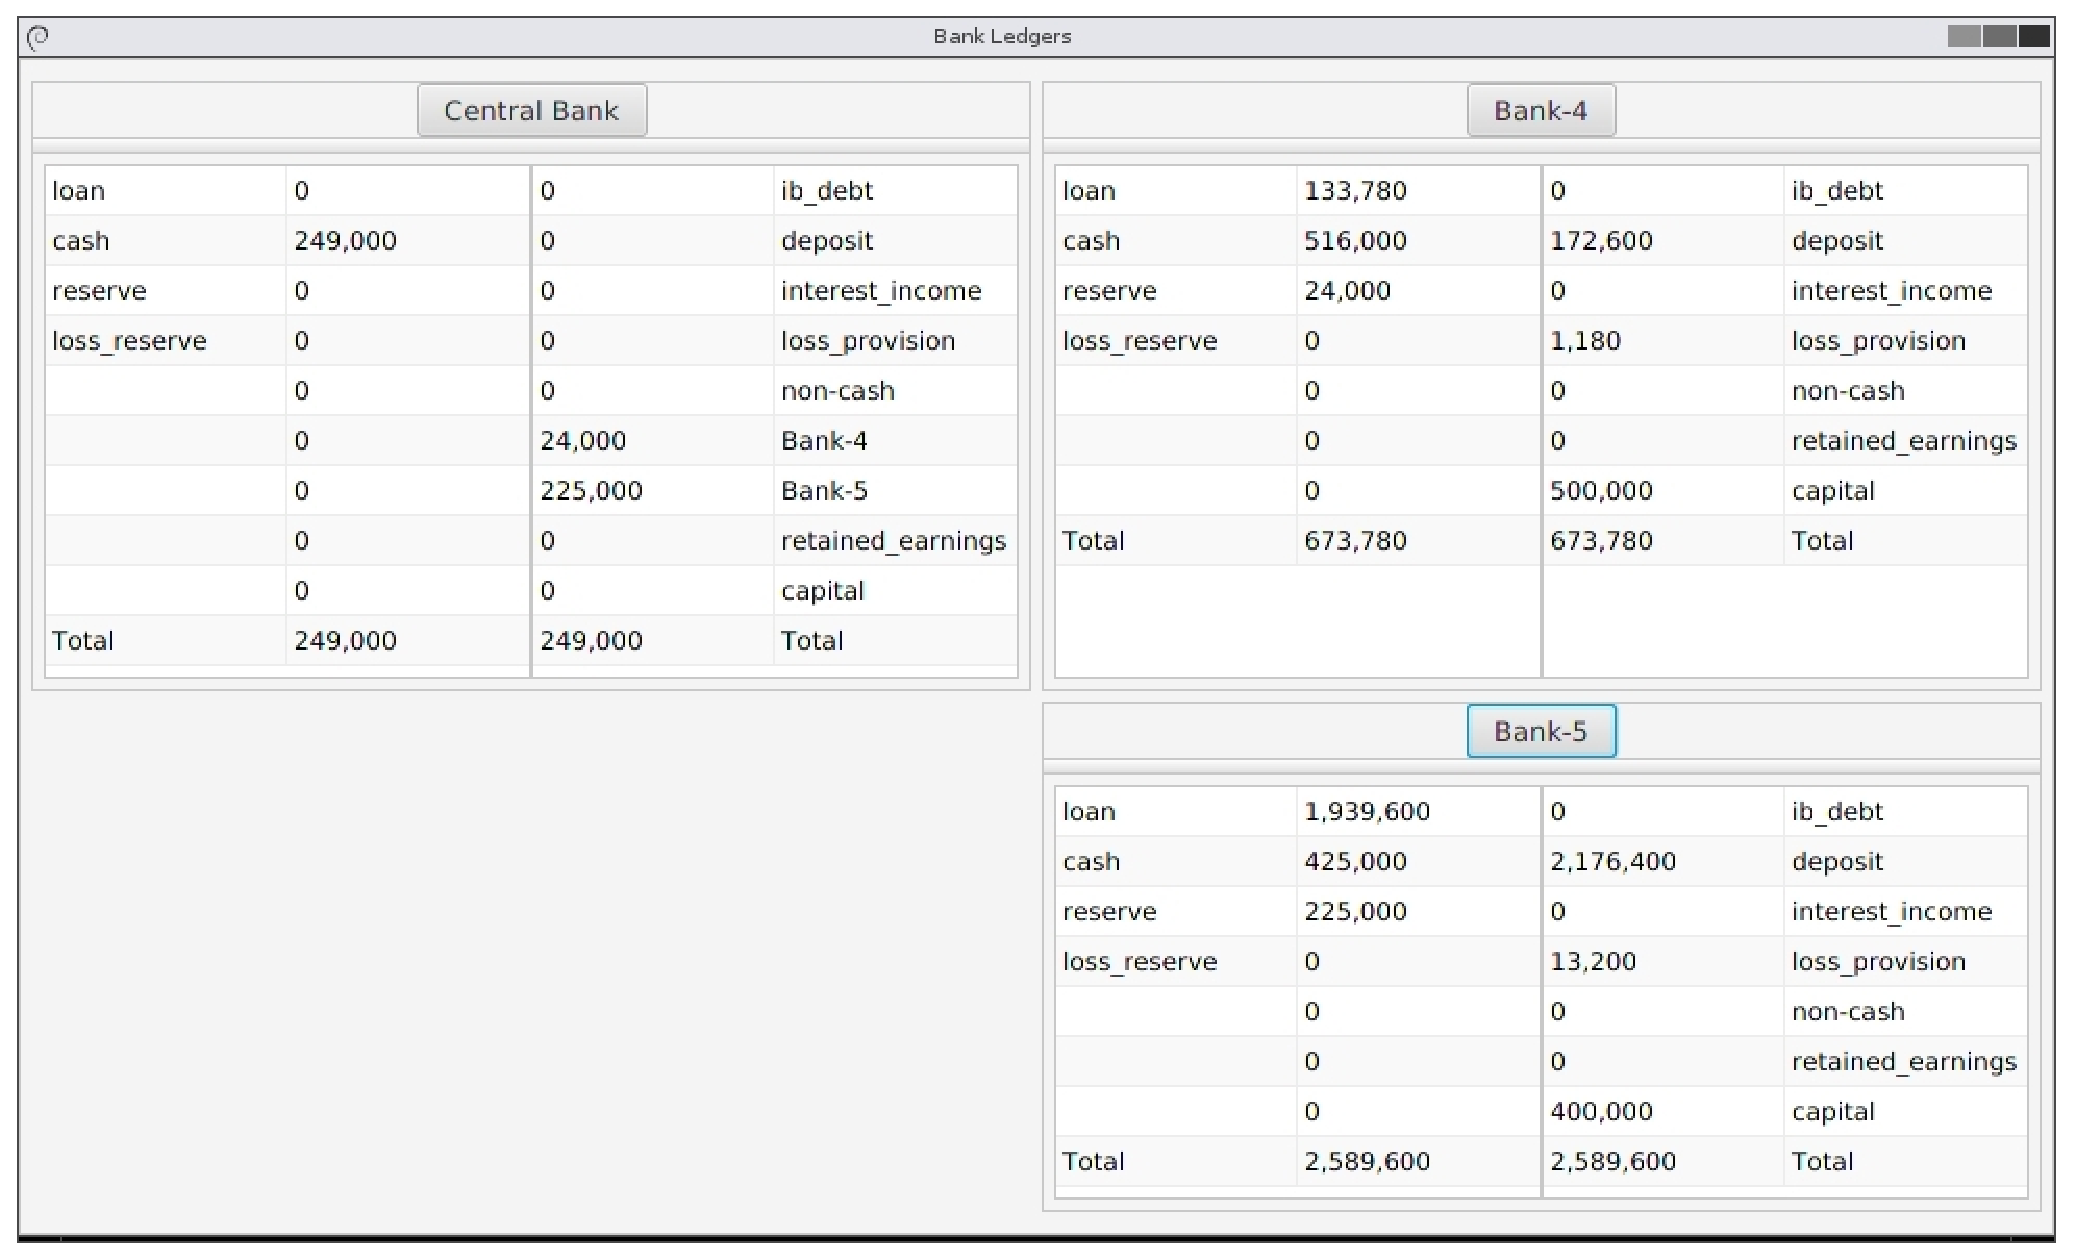
\includegraphics[width=120mm, height=60mm]{images/fig_bank_ledgers.eps}
\caption{Bank Ledger View within Threadneedle}
\label{fig:ledgerview}
\end{figure}
Figure \ref{fig:ledgerview} shows the ledger view of a 2 Bank 
simulation (Button: Show Banks) running in Threadneedle. It uses 
the accounting balance sheet presentation of bank ledgers, which places
bank assets on the right, and bank liabilities shown on the
left. While assets and liabilities are accounting definitions, 
and ledger classification usually follows intuitively, they are also 
influenced by the requirements of the double entry
book keeping rules within which they are embedded. For example,
interest income accounts
where a bank puts interest income received on its loans to customers
are classified as liabilities. 
The accounting veil for this is that it is money 'owed to 
the owners of the bank' - the alternative explanation is simply
that the double entry book keeping structure requires it to be.
\par
Setting up a bank in Threadneedle is relatively straightforward. 
All agents receive an account when they are created, and can
also receive a deposit at that time. This deposit is performed
as a cash deposit, and provides part of the liquidity for
the bank.\footnote{When banks are founded in modern economies,
the initial liquidity is provided by the investors, typically
in return for preferential shares.} The \emph{Saver} agent
can also be used to provide a cash deposit with no other side
effects.
The \emph{Investor} agent is used to specifically create capital, and
receives a Share ownership as specified. 
\par
The Central Bank Reserve and Basel Capital perecentages can be
changed for the entire banking system under the Central Bank's menu,
which also controls the base interest rate. This can be changed
at any time during the simulation with immediate effect.
\par
The long term behaviour of a bank with respect to lending and money creation
then depends quite critically on how it is setup, in particular
with respect to its cash holdings (which regulate lending
through the central bank), and its capital holdings, which under Basel
also regulate lending.
\subsection{Bank Operations}
In practice there are four key operational transactions that
embody banking operations which it is important to know,
in order to sucessfully design bank based simulations.
\footnote{A complete list of the double entry book keeping 
operations used in Threadneedle, accompanied by worked examples, can be 
found in Description of the Operational Mechanics of a Basel 
Regulated Banking System \cite{mallett.2012.2}}. 
\par
\subsubsection{Deposit Cash}
Individually, banks operate by statistically multiplexing 
physical (asset) cash, against bank liability deposits, as
shown on the ledger. When physical cash is deposited at
a bank, the double entry book keeping operation is:
\begin{table}[ht]
\centering
\begin{tabular}{ll}
debit cash & credit deposit\\
\end{tabular}
\end{table}
The physical cash deposited into the bank is now the property
of the bank, whilst a liability deposit account has been
created which is the property of the person who deposited
the cash. That person now has a claim on physical cash owned
by the bank, but not on the actual physical notes that
they deposited.
\par
\subsubsection{Transfer money to account at the same Bank}
If A, the owner of the account now wants to transfer money
to B who also has an account on the same 
ledger - say by writing a cheque, or as transfer request on
their bank account's website,  then the bank uses the book keeping operation:
\begin{table}[ht]
\centering
\begin{tabular}{ll}
debit deposit account (A) & credit deposit account (B)\\
\end{tabular}
\end{table}
Notice that since no physical cash was involved in this
transfer, and yet a monetary payment took place, this is the operation 
that gives liability deposit accounts their own status as a form of
money.
\subsubsection{Transfer money to account at another Bank}
Taking the previous example a little further. If B's
account is at another bank, then physical cash is at
least nominally involved, since physical cash\footnote{Or its
modern electronic equivalent. There is believed to still be
an element of physical transfers in some parts of the system.}
is used to transfer money \emph{between banks}.
\begin{table}[ht]
\centering
\begin{tabular}{ll}
credit cash Bank 1 & debit deposit account (A)\\
debit cash Bank 2 & credit deposit account (B)\\
\end{tabular}
\end{table}
Consequently a bank must always have some asset 
cash (or electronic equivalent) available to perform 
any required transfers between banks, as well as to meet requests
to physically withdraw cash, otherwise it is insolvent.
The general term for this in banking is \emph{liquidity}, and
sucessful banks monitor and attempt to control their liquidity status
extremely carefully, which can have surprisingly far
reaching economic consequences.
\subsubsection{Lending}
When a loan is made, the bank does the following:
\begin{table}[H]
\centering
\begin{tabular}{ll}
debit loan Borrower A & credit deposit account (A)\\
\end{tabular}
\end{table}
and when it is repaid, the money is removed as the principal
is repaid, and transferred from the depositor, to the bank
when interest is paid:
\par
\begin{table}[H]
\centering
\begin{tabular}{lll}
(1) credit loan Borrower A & debit deposit account (A) & (Repay Principal)\\
                           &                           &                \\
(2)                        & debit deposit account (A) & Pay Interest \\
                           & credit interest income    & Pay Interest \\
\end{tabular}
\end{table}
The result of banks making loans over time is to create a much larger
quantity of money represented in liability deposit accounts,
than exists as physical cash. Initially this will occur very quickly,
and then assuming regulatory controls are to some degree effective,
stabilise, as loan repayment begins to remove the money being created. The
long term behaviour of the system essentially rests on the difference
between the rate of new lending, versus loan repayment and loan default.
This is the core of
the statistical multiplexing relationship
that banks have to manage in their day to day operations, the
economic ramifications of which are to this date, extremely
poorly understood.
\subsection{Liquidity}
Liquidity - the availability of asset cash to meet demands for
withdrawals, and in particular transfers to other banks, is a 
significant issues both in simulations, and for the real economy.
Simulations that are not designed to avoid liquidity problems
will invariably enounter them very quickly, as imbalances between
banks arise due to loan repayment. While Threadneedle does implement 
interbank lending and banks will automatically attempt
to borrow from other banks to correct short term imbalances, in 
practice this will only accentuate any long term imbalances 
in liquidity flows.
\par
This is where a high level view of loans as simply flows
of money between sectors, conflicts more than a little with 
what actually occurs
within the banking mechanisms. We should also note here that
this is an area where Threadneedle is known to not accurately
simulate the behaviour of economies with small numbers of
large banks - since the precise mechanisms used within the banks
to manage their branch
banking ledgers are at this time unknown. Threadneedle uses
a single ledger for each bank.
\par
\begin{figure}[ht]
\centering
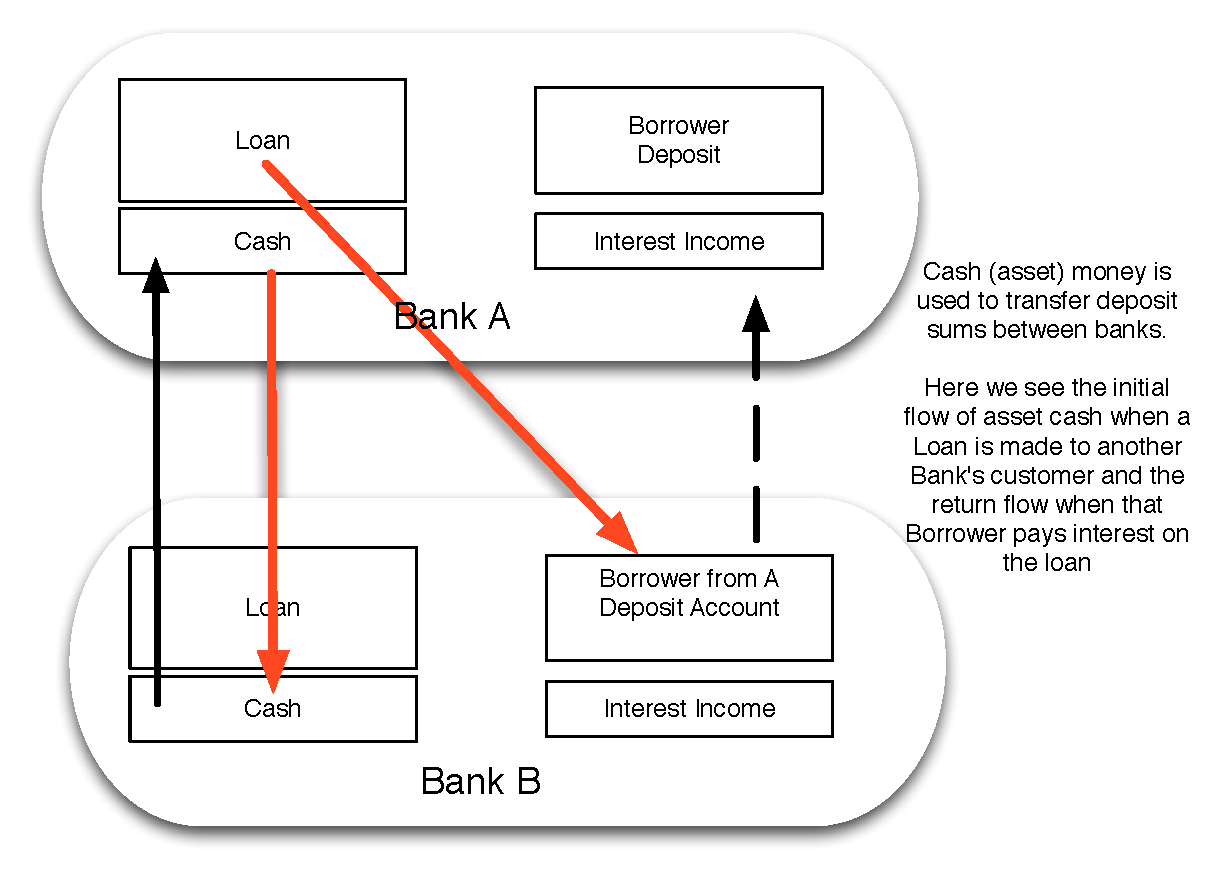
\includegraphics[width=120mm, height=60mm]{images/fig_Money-Flows.eps}
\caption{Bank Ledger View within Threadneedle}
\label{fig:money-flows}
\end{figure}
Figure \ref{fig:money-flows}
shows the asset cash transfers that accompany a customer
loan, when a bank makes a loan to a deposit holder at
another bank. For example although the interest payment is made from 
the customer's liability deposit account to Bank A's liability
interest income account, in order to perform the payment
a matching flow of cash has to flow between the banks to
register the transfer. Since loans are necessarily unbalanced - more
asset cash flows back to the bank making the loan, due to interest
payments, than Bank B receives as loan capital, over the long
term Bank B progressively loses asset money to Bank A, creating
a liquidity issue for Bank B.
\par
This is not an issue solely confined to Bank loans. Any loan
made between two parties at different banks, will inevitably
create an unbalanced liquidity flow over the long term - and
the activities of lending companies that simply use banks for
deposit funds are not under the Bank's direct control. Similarly
although lending banks strongly prefer customers to 
receive their salaries at their bank, nothing prevents 
subsequent moving of accounts. Loan
securitization - where loans are packaged and sold for example -
carries no guarantees about where in the banking system these
loans will end up, or what the influence of their long term
flows will be on the system. 
\par
These issues are important economically, because if sufficient
stress is placed on inter-bank liquidity, banks will stop making
new loans, and a credit crisis may be triggered. The key simulation
issue is that simulations must be designed to respect the liquidity
eneds of the banks, given that
even when their terms are identical, 
loans are not necessarily equivalent to each other, with respect
to the long term monetary flows they create
within the banking system, and this goes beyond
the simple issue of money creation accompanying bank loans, but not
other forms of lending. It casts light on banking not as a monolithic
entity, but rather as a subtle geographically based network process
that over time manipulates a monetary field that in many
respects is locally and regionally generated, rather than centrally
controlled.
\par
In simulations, the simplest way to test for unwanted liquidity issues
is to use a single bank for the entire simulation. Companies can
also restrict their hiring to workers using the same bank as they do,
and Regions can be used to further restrict worker availability.
Knowing that Banks are geographically organised, and make lending decisions 
based on liquidity, we believe that we are seeing issues under
simulation that are also arising within modern economies, and so
should consequently be explored.
\subsubsection{Insolvency}
Insolvency on the other hand 
is the long term inability for a bank to cover its 
obligations due to loan default, or outright theft (it can happen). 
The definition of 'long term' in this context
depends to some extent on national accounting rules and practices
around loss handling.
\par
Fundamentally, insolvency arises from defaults by customers on their loans.
Once a customer stops paying a loan, special treament and handling
by the bank of that loan/customer is typically triggered, both by its 
internal processes and as regulatory requirements. In theory, after
some number of missed or delayed payments, the loan will be closed
by the bank, any collateral associated with the bank seized,
and sold to repay the loan. If the collateral of the loan is insufficient
to cover the outstanding capital, then that amount is treated as an
expense and must be written 
off by the bank. Loan write off follows a three step process:
\begin{enumerate}
\item Deduct from loss provisions (if any)
\item Deduct from profits (if any)
\item Deduct from capital
\end{enumerate}
If the bank cannot cover the write off from 1 or 2, then it is 
effectively insolvent and ceases to be a going concern. Typically
at this point some form of government intervention occurs in order
to protect the money represented as customer deposits, since any
significant loss of liability deposit money within a banking
system potentially causes fiscal deflation.\footnote{1929 Great
Depression style.}
\par
Threadneedle currently performs steps 1 and 2 automatically, but places
the bank in runoff mode (where existing loans are repaid, but no new
ones are made) in step 3. Anything more sophisticated 
is left as an exercise to the user, since there are so many forms
intervention can take.  Loss provisions are made automatically
from interest payments, and adjusted as loan capital varies over time.
This may not be strictly accurate, since we strongly
suspect that in many banking systems toda todayy, loan fees charged by the bank
at the beginning of the loan to borrowers are providing loss provisions.
If loan payments are skipped for three (configurable) consecutive steps,
the loan is placed in write-off, any collateral is sold, and any outstanding
amount is written off according to the order above.
\par
Loss handling interacts directly with the definition of 'long term' - 
in particular how long a bank can remain technically insolvent, but
still continue as a business. Strictly, all a bank needs to do to
continue as a business is receive enough money in interest on its
loan book to cover its expenses. Since write-offs are also an expense,
in the limit banks are faced with the choice between writing off
a loan and going under, and keeping the non-performing loan on their
books and continuing in business. This is better known as the Zombie
Bank phenomena from the aftermath of the 1980's Japanese Bubble.
\par
Loss handling is consequently subject to a variety of nationally
varying regulatory requirements, primarily in order to prevent exactly
this situation. That said, in practice 
banks have a fair amount of leeway in their internal processes, with
respect to changing loan terms, re-financing, etc. in order to prevent
a loan from being placed in default. This may result in counter-intuitive
behaviour such as a bad customer receiving a favourable rate on a new
loan in order to prevent a loan default on an old one. 
\par
Viewed as a system we can make the observation that banks are extremely
vulnerable to loan losses. A back of the envelope analysis on loan
losses suggests that a bank can afford to absorb at most 1\% of its
total loan book in losses every year, before it runs into difficulties,
and this doesn't (in engineering terms) offer a lot of fault tolerance.
The partial dependency of the write-off operation on the price of the 
collateral provided with the loan
also implies a direct interaction with market based pricing mechanisms,
which may in turn be influenced directly by the banking system in 
a number of ways, for example bank lending being used as source for
market trading, and if bank 
losses and write-offs are sufficiently high that fiscal deflation 
occurs risking a potential cascade failure as lower prices trigger
more loan defaults, and more loss of money from the system. 
From a macro-economic perspective perhaps the question we should
be asking, is why the system doesn't crash more often?
\chapter{Creating Simulations}
All agents in Threadneedle must have a bank account to participate
in monetary exchange, and so  
the bank or banks that will be used for the simulation must always
be defined first. These will 
then provide the banking system within the economy. A central bank
will be created automatically for each country. By default,
each bank will also have a reserve (deposit) account at the central
bank, and this account will be used for transfers of money between
banks.
\par
In the real world, while this particular arrangement is not untypical
of small countries pre-21st century, there are many variations.
In countries such as the USA, with large numbers of small banks,
tertiary arrangements can occur, where small banks have accounts
at larger banks to provide access to inter-bank transfer facilities.
The USA is also distinguished by having 12 Federal Reserve banks,
linked together into a central banking system, rather than a single
central bank.
\par
In other countries with small numbers of large banks,  the UK for example, 
clearing has been a separate facility, arranged between banks - originating in 
manual processes where clerks would meet in order to balance
transfers between banks, and only exchange the remainder. Campbell-Kelly\cite{campbell.2010}
provides a nice comparison between the 19th century practices adopted
in the US and the UK.
\par
In the 21st century most countries are now using, or adopting, Real Time Gross
Settlement systems, which allow transfers between banks to be performed
electronically in near to real time. It is an open research question
as to what extent these mechanisms are systemically affecting.
\par
\subsection{Fractional Reserve or 'Full' Reserve}
While all banks in Threadneedle operate using double entry book keeping,
there is no requirement that they make loans. It is
possible to create a constant money economy, simply by ensuring that
banks only take deposits and do not 
lend any money. Other lending agents can be used to provide
loans if desired. Liability deposit accounts are still created, and
transfers between these accounts at different banks are still
mediated through asset cash transfers between the banks involved. 
\par
Note, it depends on the author, whether or not this in 
fact corresponds with the form of banking generically referred
to in the Economics literature as 'Full Reserve'. The unpublished
1939 paper A Program for Monetary Reform\cite{fisher.1939}
Most propononents of full reserve in fact argued for a partial
reserve - since the full reserve would only apply to demand deposits
which would still have allowed bank lending (and the associated money creation) 
to occur.
\par
In Threadneedle
unless banks are restricted to not offer loans, they will 
participate in a fractional reserve based system and make loans
subject to their individual lending decisions. By default
these are simply based on their configurable reserve requirements.
\subsection{Market Price Deterimination}
Several forms of market are available in Threadneedle, and these
are a source of ongoing experimentation. Currently a market
maker market will be automatically created for any widget
maker that is added to the simulation - this market will buy
and sell from agents with its own trading funds and attempt
to adjust price based on supply, demand and its own monetary
holdings. Market makers are restricted to not offer a price
higher than the amount of money they currently have on hand,
and by default do not borrow. Nothing prevents users adding
borrowing to their behaviour though.
\par
A very simple list market is also available where items are simply
listed in ascending order of price. No funds are attached to this
form of market.
\par
A stock market implementation is also provided which implements
a full bid/sell market where bids and sells are listed on the market
market and automatically matched when possible.
\bibliography{finance}
\raggedright
\bibliographystyle{unsrt}
%\begin{appendices}
%\chapter{Double Entry Bookkeeping}
%\chapter{Terminology}
%\paragraph{Fiscal Deflation}
%Decrease in the money supply which impacts the general price level
%causing it to drop.
%\paragraph{Productive Deflation}
%Increase in productivity which impacts the general price level
%causing it to drop.

%\end{appendices}
%\bibliography{finance}
\raggedright
\bibliographystyle{unsrt}


\end{document}
